\documentclass[10pt,landscape,a4paper]{article}
\usepackage[utf8]{inputenc}
\usepackage[english]{babel}
\usepackage[utopia,sfscaled]{mathdesign}
\usepackage{multicol}
\usepackage[top=2mm,bottom=2mm,left=2mm,right=2mm]{geometry}
\usepackage{lipsum}
\usepackage[framemethod=tikz]{mdframed}
\usepackage{microtype}
\usepackage{graphicx}
\usepackage{amsmath}
\usepackage{breqn}
\usepackage{enumitem}
\usepackage{titlesec}

\setitemize{noitemsep,topsep=0pt,parsep=0pt,partopsep=0pt}
\setlength{\parindent}{0pt}
\setlength{\parskip}{0.2\baselineskip}
\titleformat*{\section}{\footnotesize\bfseries}
\titleformat*{\subsection}{\scriptsize\bfseries}

\graphicspath{{images/}}

\DeclareMathOperator*{\argmin}{argmin}
\DeclareMathOperator*{\argmax}{argmax}

\begin{document}
\tiny
\begin{multicols*}{5}
\section{Validation}
% TODO: 2016_valid Q1 pseudocode

% TODO: different validation techniques
Model Selection:
\begin{itemize}
    \item optimization bias is small when a few models are compared
    \item optimization bias is large when a lot of models are compared
\end{itemize}


\section{Parametric \& Non-Parametric}
\begin{itemize}
    \item parametric
    \begin{itemize}
        \item fixed \# parameters
        \item more data doesn't help
    \end{itemize}
    \item non-parametric
    \begin{itemize}
        \item \# parameters grows with \(n\)
        \item more data \(\rightarrow \)  more complicated
    \end{itemize}
    \item examples:
    \begin{itemize}
        \item k-means (non-parameters)
        \item softmax multi-class classification (parametric)
        \item PCA (parametric)
        \item neural networks (parametric)
    \end{itemize}
\end{itemize}

\section{Data Standardization}
\begin{itemize}
    \item \(\mu \) = mean of \(X_j\) and \(y\), \(\sigma \) = std of \(X_j\) and \(y\)
    \item \(x_i = x_i - \frac{\mu}{\sigma}\)
    \item use the \(\mu \) and \(\sigma \) from training data on test data
\end{itemize}

\section{PCA}
\begin{dmath*}
    f(W,Z) = \sum_{i=1}^{n} \sum_{j=1}^{d} (w_j^\intercal z_i - x_{ij})^2 + \frac{\lambda_W}{2} ||W|_F^2 \frac{\lambda_Z}{2} ||Z||_F^2
\end{dmath*}
Trade-off:
\begin{itemize}
    \item reduce overfitting when \emph{both} W and Z are regularized
    % TODO: 2016 Final Q8 (d)
    % TODO: L29 s7a
\end{itemize}
PCA vs. NMF vs. Sparse PCA
\begin{itemize}
    \item PCA --- orthonormal
    \item NMF --- non-negative \& sparsity
    \item Sparse PCA --- zeros \& non-orthonormal
\end{itemize}
Note:
\begin{itemize}
    \item \(ZW = (-Z)(-W)\) (not unique)
    \item sparse PCA: \(f(Z,W) = ||ZW-X||_F^2 + \lambda_W (\sum_{j=1}^{d} ||w_j||_1) +\frac{\lambda_Z}{2} (\sum_{i=1}^{n} ||z_i||^2)\)
\end{itemize}

\section{Recommender System}
% TODO: 2017 Final Q1c

\section{Neural Networks}
\begin{dmath*}
    f(W^{(1)},W^{(2)}) = \frac{1}{2} \sum_{i=i}^{n} (w^\intercal h(W^{(2)}h(W^{(1)}x_i))-y_i)^2 + \frac{\lambda}{2}||w||^2 + \frac{\lambda_1}{2} ||W^{(1)}||_F^2 + \frac{\lambda_2}{2} ||W^{(2)}||_F^2
\end{dmath*}
\begin{itemize}
    \item \(W^1\) is \(k_1 \times d\), \(W^2\) is \(k_2 \times k_1\), and \(w\) is \(k_2 \times 1\)
    \item \(k \uparrow \) \(\rightarrow \) \(E_{train} \downarrow \text{ but } E_{approx} \uparrow \)
    \item \(\lambda \uparrow \) \(\rightarrow \) \(E_{train} \uparrow \text{ but } E_{approx} \downarrow \)
    \item depth \(\uparrow \) \(\rightarrow \) \(E_{train} \uparrow \text{ but } E_{approx} \downarrow \)
\end{itemize}

Note:
\begin{itemize}
    \item deep learning is sensitive to initialization \(\because\) it's non-convex
\end{itemize}

\subsection{Convolutional Neural Networks}
Motivation:
\begin{itemize}
    \item reduce \# parameters
    \item exploit structure in data
    \item reduce overfitting
\end{itemize}

\section{Math}
Objective functions and derivatives:
\begin{align*}
   f(x) &= \frac{1}{2}\sum\limits_{i=1}^{n} (w^\intercal x_i - y_i)^2 + \frac{\lambda}{2} \sum\limits_{j=1}^{d} w_j^2 \\
   &= \frac{1}{2} ||Xw-y||^2 + \frac{\lambda}{2} ||w||^2
\end{align*}
\begin{itemize}
    \item \(\sum\limits_{i=1}^{n} (w^\intercal x_i - y_i)^2 = \sum\limits_{i=1}^{n} r_i^2 = r^\intercal r = ||r||^2\)
    \item \(||v|| = \sqrt{\sum\limits_{j=1}^{d} v_j^2}\), \(u^\intercal v = \sum\limits_{j=1}^{d} u_j v_j\)
    \item \(||w||^2 = \sum\limits_{j=1}^{d} w_j^2 = \sum\limits_{j=1}^{d} w_j w_j = w^\intercal w \)
\end{itemize}
\begin{align*}
    f(w) &= \frac{1}{2} (Xw-y)^\intercal (Xw-y) + \frac{\lambda}{2} w^\intercal w \\
    &= \frac{1}{2} w^\intercal X^\intercal Xw - w^\intercal X^\intercal y - \frac{1}{2} y^\intercal y + \frac{\lambda}{2} w^\intercal w \\
    \nabla f(x) &= X^\intercal Xw - X^\intercal y + \lambda w = 0 \\
    & \rightarrow (X^\intercal X + \lambda I) w = X^\intercal y
\end{align*}
\begin{itemize}
    \item \(\nabla_w (c) = 0\), \(\nabla_w (w^\intercal b) = b\), \(\nabla_w (\frac{1}{2} w^\intercal A w = Aw\)
\end{itemize}
\begin{itemize}
    \item if \(f(x) = \cdots \frac{\lambda}{2} \sum\limits_{j=1}^{d} w_j v_j\), then \(f(x) = \cdots \lambda w^\intercal v\) and \(\nabla f(x) = X^\intercal Xw - X^\intercal y + \lambda v = 0\)
\end{itemize}
\begin{align*}
    f(x) &= \sum\limits_{i=1}^{n} z_i |w^\intercal x_i - y_i| + \lambda \max_j |w_j|
\end{align*}
\begin{align*}
    f(w) = ||Z(Xw - y)||_1 + \lambda ||w||_{\infty}
\end{align*}
Convexity:
\begin{itemize}
    \item \(f''(x) \geq 0 \Rightarrow \) convex
    \item a convex function multiplied by a non-negative constant is convex
    \item norms and squared norms are convex
    \item \(\exp()\) is convex
    \item sum of convex functions is convex
    \item max of convex is convex
    \item composition of a convex function and linear function is convex
    \item \emph{BUT} composition of a convex function and another convex function may not be convex
\end{itemize}
Maximum Likelihood Estimation (MLE):
\begin{itemize}
    \item minimizing NLL
    \item \(f(x) = - \sum_{i=1}^{n}\log{(p(y_i|x_i,w))}\)
    \item runtime: \(O(nd)\)
\end{itemize}

\section{Plots}
\begin{itemize}
    \item decision tree (1 variable at a time) \\
    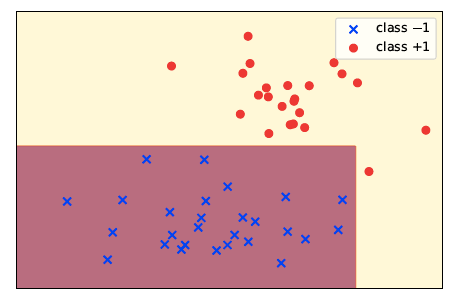
\includegraphics[scale=0.3]{decision_tree_plot}
    \item KNN with \(k=1\) \\
    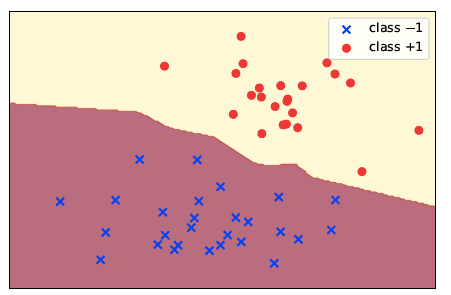
\includegraphics[scale=0.3]{knn_plot}
    \item L2-regularized logistic regression \\
    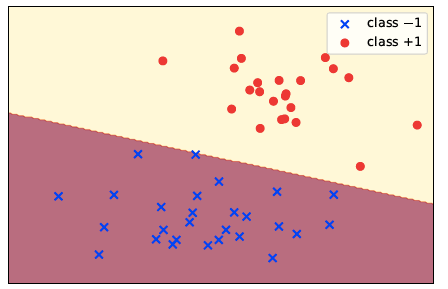
\includegraphics[scale=0.3]{l2_regularized_logistic_regression_plot}
    \item linear SVM (maximizes the margin)\\
    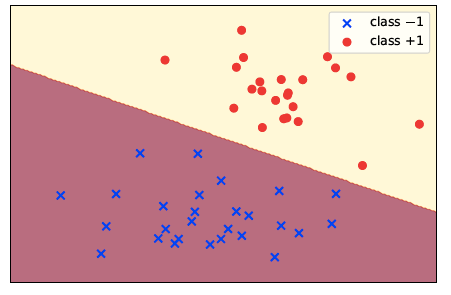
\includegraphics[scale=0.3]{linear_svm_plot}
    \item RBF SVM (blob-like boundaries) \\
    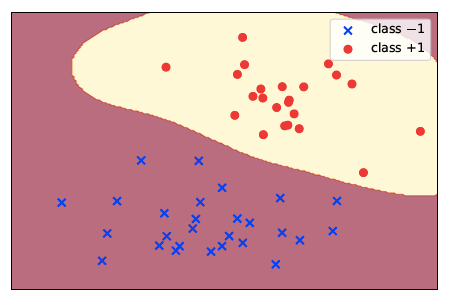
\includegraphics[scale=0.3]{rbf_svm_plot}
    \item neural network using 1 hidden layer and ReLUs \\
    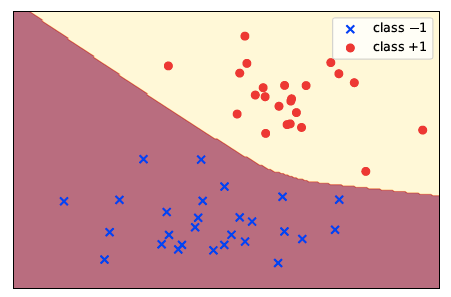
\includegraphics[scale=0.3]{neural_network_plot}
    \item non-regularized L2 norm (not robust) \\
    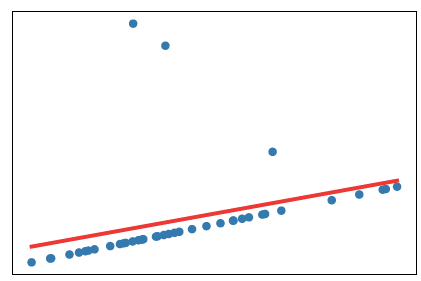
\includegraphics[scale=0.3]{non_regularized_l2_norm}
    \item regularized L2 norm (robust \(\because \) smaller slope) \\
    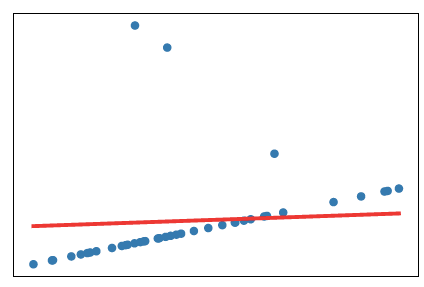
\includegraphics[scale=0.3]{regularized_l2_norm}
    \item L1 norm (robust fit \(\because \) absolute value loss) \\
    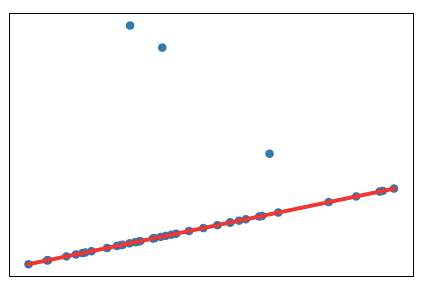
\includegraphics[scale=0.3]{l1_norm}
\end{itemize}

\section{Some Tips}
\begin{itemize}
    \item \textbf{decision stump}: computer error for different stumps then choose the one with the least error
    \item \textbf{randomness of random forest}:
    \begin{itemize}
        \item random subset of data
        \item random subset of features
    \end{itemize}
\end{itemize}

\end{multicols*}
\end{document}
